\chapter{Lecture: 12/05/2025}

$$
P(t+1) = P(t) \theta = ...
$$

$$
P(t) = P(0)\theta^t = P(0) ...
$$

???????

\begin{exampleblock}[2 States Markov Chain]
Let's consider the following example (similar to the previous one):
\vspace{-0.4em}
\begin{figure}[H]
    \centering
    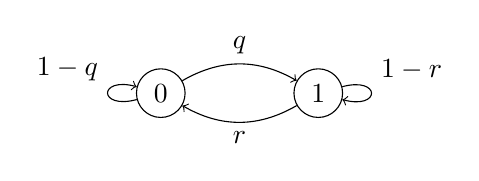
\begin{tikzpicture}
        \node[circle,draw] (s1) at (0, 0) {$0$};
        \node[circle,draw] (s2) at (2, 0) {$1$};
        % loop on s0
        \draw[->] (s1) to[loop left] node[left, yshift=0.3cm] {$1-q$} (s1);
        % transition from s0 to s1
        \draw[->] (s1) to[bend left=30] node[above] {$q$} (s2);
        % loop on s1
        \draw[->] (s2) to[loop right] node[right, yshift=0.3cm] {$1-r$} (s2);
        % transition from s1 to s0
        \draw[->] (s2) to[bend left=30] node[below] {$r$} (s1);
    \end{tikzpicture}
\end{figure}
\vspace{-1em}
We have two states ($0$ and $1$), and a probability $q$ of going from $0$ to $1$, and a probability $r$ of going from $1$ to $0$. Let $P_0(t)$ be the probability that the system is in state $0$ at time $t$, and $P_1(t)$ the probability of being in state $1$ at time $t$. The evolution of these probabilities is given by:
\vspace{0.4em}
$$
\begin{cases}
    P_0(t+1) = (1-q)P_0(t) + rP_1(t)\\
    P_1(t+1) = qP_0(t) + (1-r)P_1(t)
\end{cases}
$$
Since there are only two states, the probabilities must sum to $1$:
\vspace{0.4em}
$$
P_1(t) + P_0(t) = 1
$$

So, $P_1(t) = 1 - P_0(t)$.

\vspace{0.5em}
\textbf{Stationary (Equilibrium) Distribution:}
In the long run, the probabilities reach a steady state (stationary distribution), where $P_0(t+1) = P_0(t) = P_0^e$ and $P_1(t+1) = P_1(t) = P_1^e$. Setting the evolution equations to equilibrium, we get:
\vspace{0.4em}
$$
\begin{cases}
    P_0^e = (1-q)P_0^e + rP_1^e\\
    P_1^e = qP_0^e + (1-r)P_1^e
\end{cases}
$$
Using $P_1^e = 1 - P_0^e$, substitute into the first equation, we obtain:
\vspace{0.4em}
$$
P_0^e = \dfrac r{q+r} 
$$
Similarly:
$$
P_1^e = \dfrac q{q+r} = 1 - P_0^e
$$
\end{exampleblock}

Let's consider a Markov chain with three states: $A$, $B$, and $C$. The transitions are as follows:

\begin{figure}[H]
    \centering
    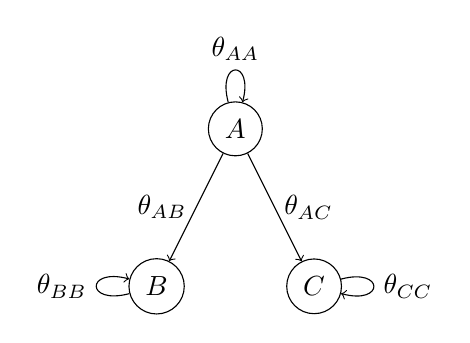
\begin{tikzpicture}
        \node[circle,draw] (A) at (1, 2) {$A$};
        \node[circle,draw] (B) at (0, 0) {$B$};
        \node[circle,draw] (C) at (2, 0) {$C$};
        \draw[->] (A) to node[left] {$\theta_{AB}$} (B);
        \draw[->] (A) to node[right] {$\theta_{AC}$} (C);
        \draw[->] (B) to[loop left] node[left] {$\theta_{BB}$} (B);
        \draw[->] (A) to[loop above] node[above] {$\theta_{AA}$} (A);
        \draw[->] (C) to[loop right] node[right] {$\theta_{CC}$} (C);
    \end{tikzpicture}
\end{figure}

Let $P_A(t)$, $P_B(t)$, $P_C(t)$ be the probabilities of being in states $A$, $B$, $C$ at time $t$. The initial state is:

$$
P(0) = (P_A(0), P_B(0), P_C(0))
$$

\textbf{Evolution Equations:}

$$
P_A(t+1) = \theta_{AA}P_A(t) ...
$$
\dots

$$
P_B(t+1) = P_B(t) + \theta_{AB}P_A(t) = P_B(t) + \theta_{AB}P_A(0) \theta^t
$$

$$
P_B(1) = P_B(0) + \theta_{AB}P_A(0)
$$

$$
P_B(2) = P_B(1) + \theta_{AB}P_A(1) = P_B(0) + \theta_{AB}P_A(0) + \theta_{AB}P_A(1)
$$

$$
P_B(t) = P_B(0) + \theta_{AB}P_A(0) \left[ 1 + \theta_{AA} + \theta_{AA}^2 + ... + \theta_{AA}^{t-1} \right]
$$

\dots

$$
P_B^{eq} = P_B(0) + P_A(0) \dfrac{\theta_{AB}}{1-\theta_{AA}}
$$

$$
P_C^{eq} = P_C(0) + P_A(0) \dfrac{\theta_{AC}}{1-\theta_{AA}}
$$

$$
det(\theta - \lambda z) = \begin{array}{|ccc|}
    \theta_{AA} - \lambda & \theta_{AB} & \theta_{AC} \\
    0 & 1- \lambda & 0\\
    0 & 0 & 1- \lambda
\end{array} = 0
$$

...

$$
P^e = H\; \text{Diag}[1, 0, ..., 0] H^{-1}P(0)
$$

and we have:
$$
P^e = W P^e
$$

Properties of $W$:

\begin{enumerate}
    \item At least $\lambda_1 = 1$
    \item $|\lambda_j| \leq 1$ for all $j$
    \item $\sum_{j=1}^n V_j = 0$
\end{enumerate}

where $V_j$ is the eigenvector of $W$ associated with $\lambda_j$.

\dots

$$
W V_j = \lambda_j V_j
$$

$$
\sum_{C = 1}^n W_{RC}(V_j)_C = \lambda_j (V_j)_R
$$

$$
\sum_{R = 1}^n \sum_{C = 1}^n W_{RC}(V_j)_C = \lambda_j \left( \sum_{R = 1}^n  (V_j)_R \right)
$$

$$
\underbrace{\sum_{C = 1}^n (V_j)_C}_{S} = \lambda_j \bigg( \underbrace{\sum_{R = 1}^n  (V_j)_R}_{S} \bigg)
\quad \Rightarrow \quad
(1 - \lambda_j)S = 0
$$

\dots

$$
P^{eq} = H \; \text{Diag}[1, 0, ...]P(0)
$$

$$
P(0) = C_2 V_1 + \sum_{j = 2}^N C_j V_j
$$

\dots

$$
P(0) =U_1 + \sum_{j = 2}^N C_j V_j
$$

Where $U_1$ is the normalized vector

\dots

$$
P(0) = C_1 V_1 + C_2 V_2 + \sum_{j = 3}^N C_j V_j
$$

$$
1 = C_1 \|{V_1}\|_1 + C_2 \|{V_2}\|_1 
\quad \Rightarrow \quad
C_2 = \dfrac{1 - C_1 \|{V_1}\|_1}{\|{V_2}\|_1}
$$

$$
P(0) = C_1 U_1 + (1-C_1) U_2 + \sum_{j = 3}^N C_j U_j
$$

$$
P(t) = W^t P(0) = C_1 U_1 + (1-C_1) U_2 + \sum_{j = 3}^N C_j \lambda_j^t V_j
$$

So $C_1$ depends on the initial state $P(0)$:

$$
\boxed{C_1 = P(P(0))}
$$

\dots

$$
P(t) = C_1 P(0) U_1 + (1-C_1 (P(0)))U_2 + \sum_j C_j \lambda_j^t V_j
$$

$$
P^e = C_1 U_1 + (1-C_1) U_2
$$

---

If we have a problem and we want to study the time of remaining in a state $A$, we can simply consider all the transitions from $A$ to other states as a single transition from $A$ to a new state $B$ (which represents the rest of the world), and it is given by the sum of all the initial transitions.

So we have now only 2 transitions: the loop from $A$ to itself, and the new $AB$ transition.

We have:

$$
x(0) = A,
\qquad \qquad
P(0) = (1, 0)
$$

$$
P_A(t) = \theta_{AA}^t 
$$

\dots

$$
P_A(T) = \theta_{AB} = \theta_{AB} \theta_{AA}^t  = (1- \theta_{AA})\theta_{AA}
$$

So the average value of $T$ is:

$$
\langle T \rangle = \sum T \theta_{AB} \theta_{AA}^t = \theta_{AB} \sum_{t=0}^{\infty} t \theta_{AA}^t
$$

$$
= \theta_{AB} \left[ 0 + \theta_{AA}^1 + 2 \theta_{AA}^2 + 3 \theta_{AA}^3 \right] = \theta_{AB} \theta_{AA} \left[ 1 + 2 \theta_{AA} + 3 \theta_{AA}^2 + ... \right]
$$

$$
= \theta_{AB} \theta_{AA} \dfrac{\dd}{\dd \theta_{AA}} \left[ -1 + 1 + \theta_{AA} + \theta_{AA}^2 + ... \right]
$$

$$
= \theta_{AB} \theta_{AA} \dfrac{\dd}{\dd \theta_{AA}} \left[ \dfrac{1}{1-\theta_{AA}} \right]
$$

